\documentclass[a4paper]{article}
\usepackage[margin=2cm]{geometry}
\usepackage{tikz}
\usepackage{float}
\usepackage{xcolor}
\usepackage{amssymb}
\usepackage{amsmath}

\usetikzlibrary{shapes.geometric}
\usetikzlibrary{intersections}
\usetikzlibrary{angles, quotes}

\begin{document}
\subsubsection*{Two Relations}
\begin{itemize}
  \item Correlation
  \item Markov
\end{itemize}
\subsubsection*{Joint Distribution}
\begin{itemize}
  \item \textbf{Understanding}:
    $$
    f_{XY}(x, y) = f_X(x)f_Y(y)
    $$

  \item \textbf{Cognition}:

    \begin{figure}[H]
      \begin{minipage}{0.4\textwidth}
        \begin{tikzpicture}
          \draw[->] (-2,0) -- (2,0) node[anchor=west]{x};
          \draw[->] (0,-2) -- (0,2) node[anchor=south]{y};
          \draw(-1.5, -1) rectangle (1.5, 1);
          \draw[ultra thick](1, -1) -- (1, 1);
        \end{tikzpicture}
        \caption{Independent}
      \end{minipage}
      \hfill
      \begin{minipage}{0.58\textwidth}
        \begin{tikzpicture}
          \draw[->] (-2,0) -- (2,0) node[anchor=west]{x};
          \draw[->] (0,-2) -- (0,2) node[anchor=south]{y};
          \node[draw, circle, minimum size=2cm] (c1) at (0,0) {};
          \draw[ultra thick] (c1.45) -- (c1.-45);
        \end{tikzpicture}
        \caption{Non-Independent, Non-Correlated}
      \end{minipage}
    \end{figure}
\end{itemize}

\subsubsection*{Correlation}

Trend:
\begin{figure}[H]
\centering
\begin{tikzpicture}
  \draw[->] (-2,0) -- (2,0) node[anchor=west]{x};
  \draw[->] (0,-2) -- (0,2) node[anchor=south]{y};
  \node[draw, ellipse, minimum width=3cm, minimum height=1cm, rotate=30, name path=ell] (e1) at (0,0) {};
  \path[name path=line] (0.5, -1) -- (0.5, 1);
  \draw [ultra thick, name intersections={of=ell and line}] 
    (intersection-1) -- (intersection-2);
  \draw[dashed] (e1.0) -- (e1.180);
\end{tikzpicture}
\caption{Non-Independent, Correlated}
\end{figure}
\subsubsection*{Correlation: Metric(Distance) between $X$ and $Y$}
\begin{itemize}
  \item Mean Square: $d(X, Y) = (E(X-Y)^2)^{\frac 12}$
    $$E(X-Y)^2 = E(X)^2 + E(Y)^2 + 2{\color{red}E(XY)}$$
  \item $E(XY) = \int_{-\infty}^{\infty}\int_{-\infty}^{\infty}xyf_{X,Y}(x,y)dxdy$\quad Correlation
    \begin{itemize}
      \item $E(XY) = 0$\quad Uncorrelated
      \item If $X$ and $Y$ are independent, then $E(XY) = E(X)E(Y)$.
    \end{itemize}
  \item Another style: $E(X-E(X))(Y-E(Y))=E(XY)-E(X)E(Y)$
\end{itemize}
Independence is stronger then Correlation.

e.g. $\theta\sim U(0, 2\pi), X=\cos(\theta), Y=\sin(\theta)$
\subsubsection*{Correlation Coefficient}

$$|E(XY)/(EX^2EY^2)^{\frac 12}| \leq 1$$

Cauchy-Schwarz Inequality: $$|E(XY)|\leq(EX^2EY^2)^{\frac 12}$$

\subsubsection*{Inner Product: $XY$, $\langle X, Y\rangle$}

Three Properties:
\begin{itemize}
  \item $\langle x, x\rangle \geq 0$, $\langle x, x\rangle =0\Leftrightarrow x=0$
  \item $\langle x,y\rangle=\langle y,x\rangle$
  \item $\langle x, \alpha y+\beta z\rangle = \alpha\langle x, y\rangle + \beta\langle x, z\rangle\\ \langle \alpha x + \beta y, z\rangle =\alpha\langle x,z\rangle + \beta\langle y,z\rangle $
\end{itemize}

$$|\langle X, Y\rangle|\leq|\langle X,X\rangle\langle Y,Y\rangle|^{\frac 12}$$

\textbf{Proof}:
$$g(\alpha)=\langle \alpha X+Y,\alpha X+Y\rangle\geq 0$$

Other formats:

$$(\sum_{k=1}^k x_ky_k)^2 \leq (\sum_{k=1}^n x_k^2)(\sum_{k=1}^ny_k^2)$$

$$(\int_a^b f(x)g(x)dx)^2\leq\int_a^bf^2(x)dx\int_a^bg^2(x)dx$$

Geometrical View: Inner product represents angle.

$$\angle(X, Y)=\arccos \left(\frac{\langle X,Y\rangle}{(\langle X,X\rangle\langle Y,Y\rangle)^{\frac 12}}\right)=\arccos \left(\frac{EXY}{(EX^2EY^2)^{\frac 12}}\right)$$

\textbf{Understanding}:
$$\min E(\alpha X-Y)^2 \Rightarrow \frac{d}{d\alpha}E(\alpha X-Y)^2\Rightarrow\alpha = \frac{EXY}{EX^2}$$
\textbf{Cognition}: Projection
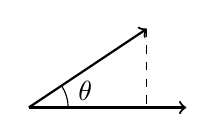
\begin{tikzpicture}
  \coordinate (O) at (0,0);
  \coordinate (A) at (2,0);
  \coordinate (B) at (1.5,1);

  \draw[->, thick] (O) -- (A);
  \draw[->, thick] (O) -- (B);
  \draw[dashed] (1.5,1) -- (1.5,0);

  \pic [draw, "$\theta$", angle eccentricity=1.5] {angle = A--O--B};
\end{tikzpicture}
$$\|Y\|\cdot \cos\theta=\|Y\|\cdot\frac{\langle X,Y\rangle}{\|X\| \|Y\|}=\frac{\langle X,Y\rangle}{\|X\|}=\frac{\langle X,Y\rangle}{\|X\|^2}\|X\|$$

\subsubsection*{Stochastic Processes}
$X(t)$: a stochastic process, get different r.v. in different time, which is not a function, see below:
$$X(\omega, t), \omega\in\Omega, t\in\mathbb{R}$$
$\omega$ is one of the sample points.

$\forall t, s\in\mathbb{R}$, calculate $E(X(t)X(s))$, then we can find the relation between these two moments, such as stocks.
\subsubsection*{Correlation Function $R_X(t,s)$}
$$\forall t, s\in\mathbb{R}, E(X(t)X(s))=R_X(t,s)$$

Binary relation: the simplest case, but can be simpler.

\subsubsection*{Wide-Sense Stationary, Invariance}
$$\forall T, R_X(t+T, s+T) = R_X(t,s)$$
or $$E(X(t))=m(t)=m$$
\textbf{Cognition}:
$$R_X(t,s)=R_X(t-s)=R_X(\eta), \eta=t-s$$
single variable.

\subsubsection*{Phase Modulation}
$$X(t)=\cos(2\pi f_0t + \theta), \theta\sim U(0, 2\pi)$$
\textbf{Understanding}:
$$E(X(t)) = \frac{1}{2\pi}\int_0^{2\pi}\cos(2\pi f_0t + \theta)d\theta=0$$
$$\begin{aligned}
  R_X(t,s)=E(X(t)X(s)) &=\frac{1}{2\pi}\int_0^{2\pi}\cos(2\pi f_0t + \theta)\cos(2\pi f_0s + \theta)d\theta \\ &=\frac{1}{4\pi}\int_0^{2\pi}\left(\cos(2\pi f_0(t+s) + 2\theta)\right) + \cos(2\pi f_0(t-s))d\theta \\ &=\frac 12\cos(2\pi f_0(t-s))
\end{aligned}$$

\subsubsection*{Random Telegraph Signal}

Random flip.

Discrete Possion Distribution:
$$P(X=k)=\frac{(\lambda t)^k}{k!}\exp(-\lambda t)$$

Between moments s and t, there is $k$ flip times $P([s, t]=k)$.

$$\begin{aligned}
  R_X(t,s)&=E(X(t)X(s)) \\
          &=P(X(t)X(s)>0) - P(X(t)X(s)<0)\\
          &=P([s,t]\text{ is even}) - P([s,t]\text{ is odd})\\
          &=\sum_{\text{k is even}}P([s,t]=k) -\sum_{\text{k is odd}}P([s,t]=k) \\
          &=\sum_{\text{k is even}}\frac{\lambda(t-s)^k}{k!}\exp(-\lambda(t-s)) - \sum_{\text{k is odd}}\frac{\lambda(t-s)^k}{k!}\exp(-\lambda(t-s))\\
          &=\frac 12\exp(-\lambda(t-s))\Bigl(\bigl(\exp(\lambda(t-s))+\exp(-\lambda(t-s))\bigr)-\bigl(\exp(\lambda(t-s))-\exp(-\lambda(t-s))\bigr)\Bigr)\\
          &=\exp(-\lambda(t-s))\Rightarrow \exp(-\lambda|t-s|)
\end{aligned}$$
\end{document}
